The structure of PVX was determined by Grinzato et al., up to a resolution of $\SI{2.2}{\angstrom}$ \cite{Grinzato2020}. The structural data was made available through the PDB, as a file containing $13$ consecutive protein subunits, forming one-and-a-half cycles of the helix. Notably, structural determination was not possible for the 29 amino acids long N-terminal domain, due to its flexibility. The N-terminal domain is relevant for the particle's structure and assembly. In experiments by \cite{del22_rigid}, it was found that while a deletion of the 22 N-terminal amino acids still leaves the virus infectious, the morphology of the particles changes from the wild type. The structure-guided computational design process will only be used to design the rigid part of the protein, the N-terminal domain will however be fused to the constructs in the end. 

The following chapters require a flexible way to use the symmetry of PVX, such as the ability to generate different configurations of monomers (e.g. a $3 \times 3$ neighborhood of monomers), or the ability to dynamically enforce this symmetry during symmetry-guided prediction with AlphaFold (\autoref{ch:alphafold}) or symmetry-guided design with RFdiffusion (\autoref{ch:rfdiffusion}). Therefore, this section discusses the computation of the symmetry relationship between consecutive monomers, and how it can be applied to generate new configurations of monomers.

Let $\{\vec{\mathbf{r}}_{j,i}^{\,\text{original}}\}$ denote the backbone atom positions of chain $j$ in the original PDB file, and let $\{\vec{\mathbf{r}}_{j}^{\,\text{original}}\}$ be their arithmetic mean. 

We choose $T_0 = (I_3, \vec{\mathbf{r}}_A^{\,\text{original}})$ as our new origin, centered on chain $A$. The backbone atom coordinates in this frame are denoted by $\vec{\mathbf{r}}_{j,i}$, and we have
\begin{equation}
    \vec{\mathbf{r}}_{j,i} = T_0^{-1} \circ \vec{\mathbf{r}}_{j,i}^{\,\text{original}} = \vec{\mathbf{r}}_{j,i}^{\,\text{original}} - \vec{\mathbf{r}}_{A}^{\,\text{original}}
\end{equation}

The frames of all other chains in these coordinates are computed as the optimal rigid body transform to align the chain with A. That is,
\begin{equation}
T_j = \underset{T \in \mathrm{SE}(3)}{\arg\min} \sum_i \left\| T\circ\vec{\mathbf{r}}_{A,i} - \vec{\mathbf{r}}_{j,i} \right\|^2
\end{equation}

Using the Kabsch algorithm \cite{Lawrence_2019}, $T_j$ can be computed as $T_j = (R_j, \vec{\mathbf{t}}_j)$, where 
\begin{equation}
    \vec{\mathbf{t}}_j= \vec{\mathbf{r}}_j - R_j\vec{\mathbf{r}}_A =\vec{\mathbf{r}}_j
\end{equation}    
since $\vec{\mathbf{r}}_A=\vec{\mathbf{0}}$, and $R_j \in \mathrm{SO}(3)$ minimizes 
\begin{equation}
\sum_{i} \left\| R_j(\vec{\mathbf{r}}_{A,i} - \vec{\mathbf{r}}_{A})  - (\vec{\mathbf{r}}_{j,i} - \vec{\mathbf{r}}_{j})\right\|
\end{equation}
Following the Kabsch Algorithm, $R_j$ can be computed via the singular value decomposition 
\begin{equation}
    (\vec{\mathbf{r}}_{A,i} - \vec{\mathbf{r}}_{A})^T  \cdot (\vec{\mathbf{r}}_{j,i} - \vec{\mathbf{r}}_{j}) = U\Sigma V^T \\
\end{equation}
as 
\begin{equation}
R_j = V\cdot \operatorname{diag}(1, 1, d)\cdot U^T
\end{equation}
where $d = \det(U)\det(V)$ corrects for a potential reflection in the orthogonal matrices $U$ and $V$.

With all frames $T_j$ expressed in the same coordinate system, we can compute the relative transform
\begin{equation}
T_{j\rightarrow j+1} = (R_{j\rightarrow j+1}, \vec{\mathbf{t}}_{j\rightarrow j+1}) = T_j^{-1}\circ T_{j+1}
\end{equation}
Given the symmetry of the viral coat structure, these transforms are expected to be equal. The average relative transform $T_R = (R_R, \vec{\mathbf{t}}_R)$ is computed by choosing $\vec{\mathbf{t}}_R$ as the mean over $\{\vec{\mathbf{t}}_{j\rightarrow j+1}\}$ and choosing $R_R \in \mathrm{SO}(3)$ as the rotation matrix closest to the average over all $R_{j\rightarrow j+1}$, that is $R_R=UV^T$ where $U\Sigma V^T = \frac{1}{n}\sum_j R_{j\rightarrow j+1}$ \cite{Sarabandi2023} (given the similarity of the $\{R_{j\rightarrow j+1}\}$, no reflection can arise by continuity). 

The individual rotations $R_{j\rightarrow j+1}$ had standard deviation $\Delta R_R = \SI{0.004}{\radian}$ in geodesic distance, and the individual translations had standard deviation $\Delta \mathbf{t}_R = \SI{0.04}{\angstrom}$. $R_R$ closely resembles a pure rotation around the z-axis $R_Z(\theta)$, with an angle of $\theta = \SI{-0.707}{\radian}$. The deviation is $d(R_R, R_Z(\theta)) = \SI{0.005}{\radian}$. This value of $\theta$ corresponds to a left-handed helix with $8.89$ subunits per turn. The computed rise is $\mathbf{t}_z=\SI{3.87}{\angstrom}$ per subunit, resulting in a helical pitch (rise per turn) of $\SI{34.4}{\angstrom}$. These values are mostly consistent with the ones stated in \cite{Grinzato2020} (rise $\SI{3.96}{\angstrom}$, rotation of $\SI{0.707}{\radian}$, $8.9$ copies per turn, helical pitch $\SI{35.2}{\angstrom}$). However, the authors emphasize the slight difference in the helical pitch of $\SI{35.2}{\angstrom}$ compared to that of similar flexible filamentous plant viruses (PepMV, BaMV, and PapMV), for which the helical pitch ranges from $\SI{34.3}{\angstrom}$ to $\SI{34.6}{\angstrom}$. According to the calculations above, the helical pitch in the PDB entry (which the authors produced through multiple cycles of real space refinement) differs from the original helical parameters fitted to the cryo-EM data and falls into the range of the other plant viruses, thereby potentially diminishing the significance of the reported pitch deviation. 

\begin{table}
    \centering
    \caption{\textbf{Visualization and chain indices of different monomer configurations}, generated based on the average relative transform $T_R$. The blue chain has index $0$, the coordinates for the other chains are computed as $T_R^j \circ \vec{\mathbf{r}}_{A,i}, j \in I$. The generated monomer configurations will be used to create inputs for the algorithms in the following sections. }
    \begin{tblr}{colspec={Q[c]Q[c]Q[c,h]}}
        \hline
        \textbf{Type} & \textbf{Indices} & \textbf{Visualization} \\
        \hline
        Helical & $I=\{0, ..., 12\}$ & 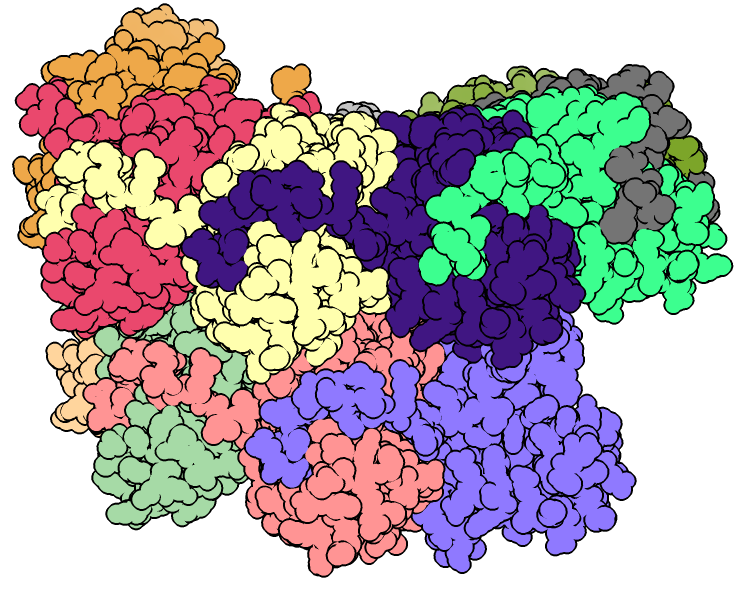
\includegraphics[height=2.5cm]{pvx_slices/vis_helix.png} \\
        \hline
        3x3 & $I=\{0, \pm 1, \pm 8, \pm 9, \pm 10 \}$ & 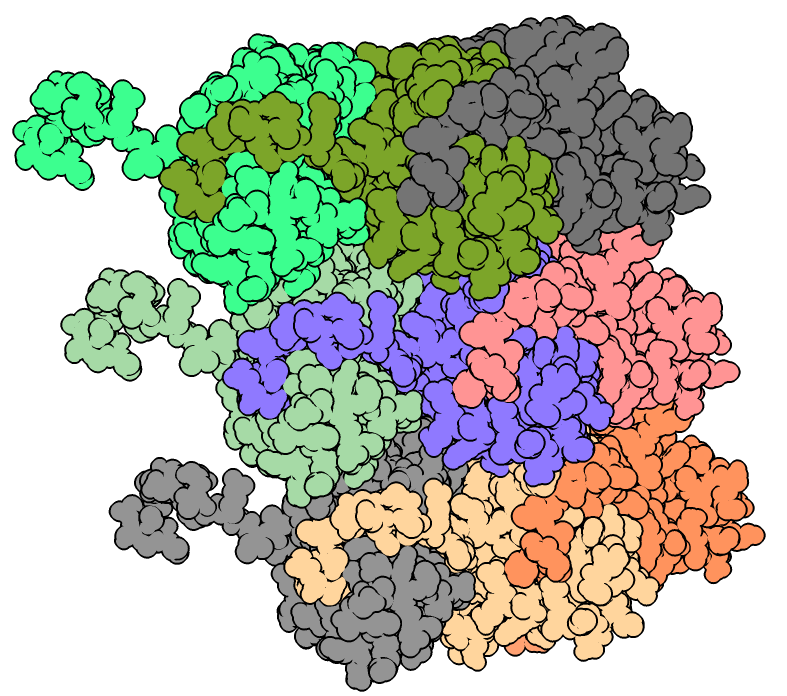
\includegraphics[height=2.5cm]{pvx_slices/vis_3x3.png} \\
        \hline
        Trimer & $I=\{0, \pm 1\}$ & 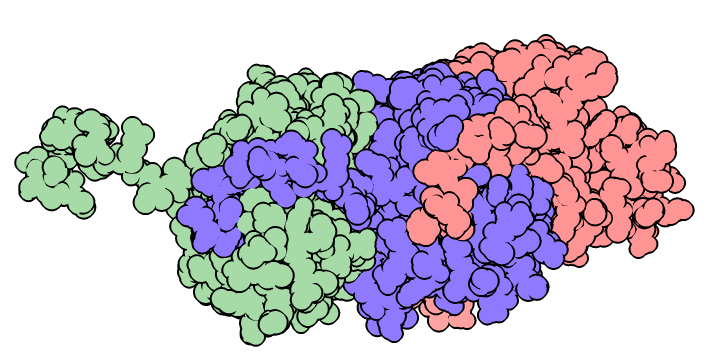
\includegraphics[height=1.5cm]{pvx_slices/vis_trimer.png} \\
        \hline
        Pentamer & $I=\{0, \pm 1, \pm 9 \}$ & 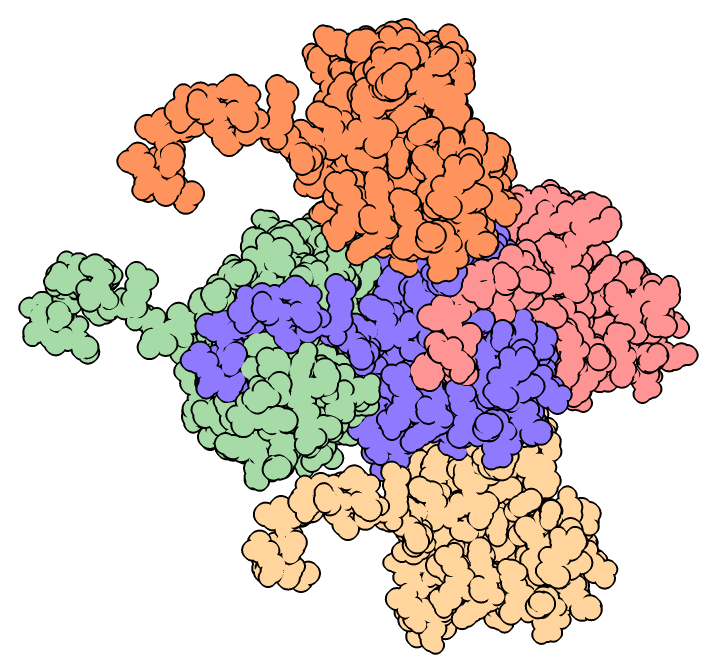
\includegraphics[height=2.5cm]{pvx_slices/vis_pentamer.png} \\
        \hline
    \end{tblr}
    \label{tab:01_symmetry}
\end{table}

Given the relative transform $T_R$, model coordinates can be reconstructed based on the coordinates of the monomer $A$ according to 

\begin{equation}\label{eq:01_symmetry}
\vec{\mathbf{r}}_{j,i}^{\,\text{original}} = T_0 \circ T_R^j \circ \vec{\mathbf{r}}_{A,i}
\end{equation}

Using \autoref{eq:01_symmetry}, four different configurations of monomers are generated and used throughout the following sections (\autoref{tab:01_symmetry}). A helical configuration consisting of thirteen consecutive monomers, a three-by-three neighborhood of nine monomers, a trimer consisting of three consecutive monomers, and a pentamer consisting of five monomers arranged in a cross-shape. 

Despite the small standard deviation of $T_R$, the deviation of individual atom positions in the helical thirteen-monomer reconstruction compared to the data from the pdb entry reaches up to $\SI{0.8}{\angstrom}$. This is due to lever effects caused by small deviations in the rotation. The difference in structure introduces no new clashes, but slightly reduces the contacts by $\SI{2}{\percent}$, as computed with ChimeraX \cite{ChimeraX2023}.